%%% Template originaly created by Karol Kozioł (mail@karol-koziol.net) and modified for ShareLaTeX use

\documentclass[a4paper,11pt]{article}

\usepackage[T1]{fontenc}
\usepackage[utf8]{inputenc}
\usepackage{graphicx}
\usepackage{xcolor}

\renewcommand\familydefault{\sfdefault}
\usepackage{tgheros}

\usepackage{amsmath,amssymb,amsthm,textcomp}
\usepackage{enumerate}
\usepackage{multicol}
\usepackage{tikz}

\usepackage{geometry}
\geometry{left=25mm,right=25mm,%
bindingoffset=0mm, top=20mm,bottom=20mm}


\linespread{1.3}

\newcommand{\linia}{\rule{\linewidth}{0.5pt}}

% custom theorems if needed
\newtheoremstyle{mytheor}
    {1ex}{1ex}{\normalfont}{0pt}{\scshape}{.}{1ex}
    {{\thmname{#1 }}{\thmnumber{#2}}{\thmnote{ (#3)}}}

\theoremstyle{mytheor}
\newtheorem{defi}{Definition}

% my own titles
\makeatletter
\renewcommand{\maketitle}{
\begin{center}
\vspace{2ex}
{\huge \textsc{\@title}}
\vspace{1ex}
\\
\linia\\
\@author \hfill \@date
\vspace{4ex}
\end{center}
}
\makeatother
%%%

% custom footers and headers
\usepackage{fancyhdr}
\pagestyle{fancy}
\lhead{}
\chead{}
\rhead{}
\lfoot{}
\cfoot{}
\rfoot{Page \thepage}
\renewcommand{\headrulewidth}{0pt}
\renewcommand{\footrulewidth}{0pt}
%

% code listing settings
\usepackage{listings}
\lstset{
    language=lisp,
    basicstyle=\ttfamily\small,
    aboveskip={1.0\baselineskip},
    belowskip={1.0\baselineskip},
    columns=fixed,
    extendedchars=true,
    breaklines=true,
    tabsize=4,
    prebreak=\raisebox{0ex}[0ex][0ex]{\ensuremath{\hookleftarrow}},
    frame=lines,
    showtabs=false,
    showspaces=false,
    showstringspaces=false,
    keywordstyle=\color[rgb]{0.627,0.126,0.941},
    commentstyle=\color[rgb]{0.133,0.545,0.133},
    stringstyle=\color[rgb]{01,0,0},
    numbers=left,
    numberstyle=\small,
    stepnumber=1,
    numbersep=10pt,
    captionpos=t,
    escapeinside={\%*}{*)}
}

%%%----------%%%----------%%%----------%%%----------%%%

\begin{document}
\title{El Despegue - Tarea \textnumero{} 02}

\author{Enrique Giottonini}

\date{OKTOBERFEST}

\maketitle

\section*{Problema 5}
La llamada (bundle ’(”a” ”b” ”c”) 0) es un buen uso de bundle ? ¿qué produce?
¿por qué? \\ \\
Sea $\gamma = (bundle\, s\, n)$ donde $s$ es una lista de caracteres y $n$ el tamaño de los trozos entonces:
\[ (length\,\gamma) = \Big \lceil \dfrac{length(s)}{n}\Big \rceil\]
Por lo que no tiene sentido que $n$ sea igual a 0. En la implementacion de <bundle> esto se refleja en la llamada recursiva.

\begin{lstlisting}[title=bundle]
(define (bundle s n)
  (cond
    [(null? s) null]
    [else
     (cons (implode (take s n))
           (bundle (drop s n) n))]))
\end{lstlisting}

$(drop \,s \,n) = s$ si $n=0$ por lo que la llamada recursiva  en $(bundle\, s\, 0)$ entraria en un loop infinito.
\newpage
\section*{Problema 9}
Dibuja un diagrama como el de la figura anterior($<quicksort>$) pero para la lista ’(11 9 2 18 12
14 4 1) .

\begin{figure}[ht]
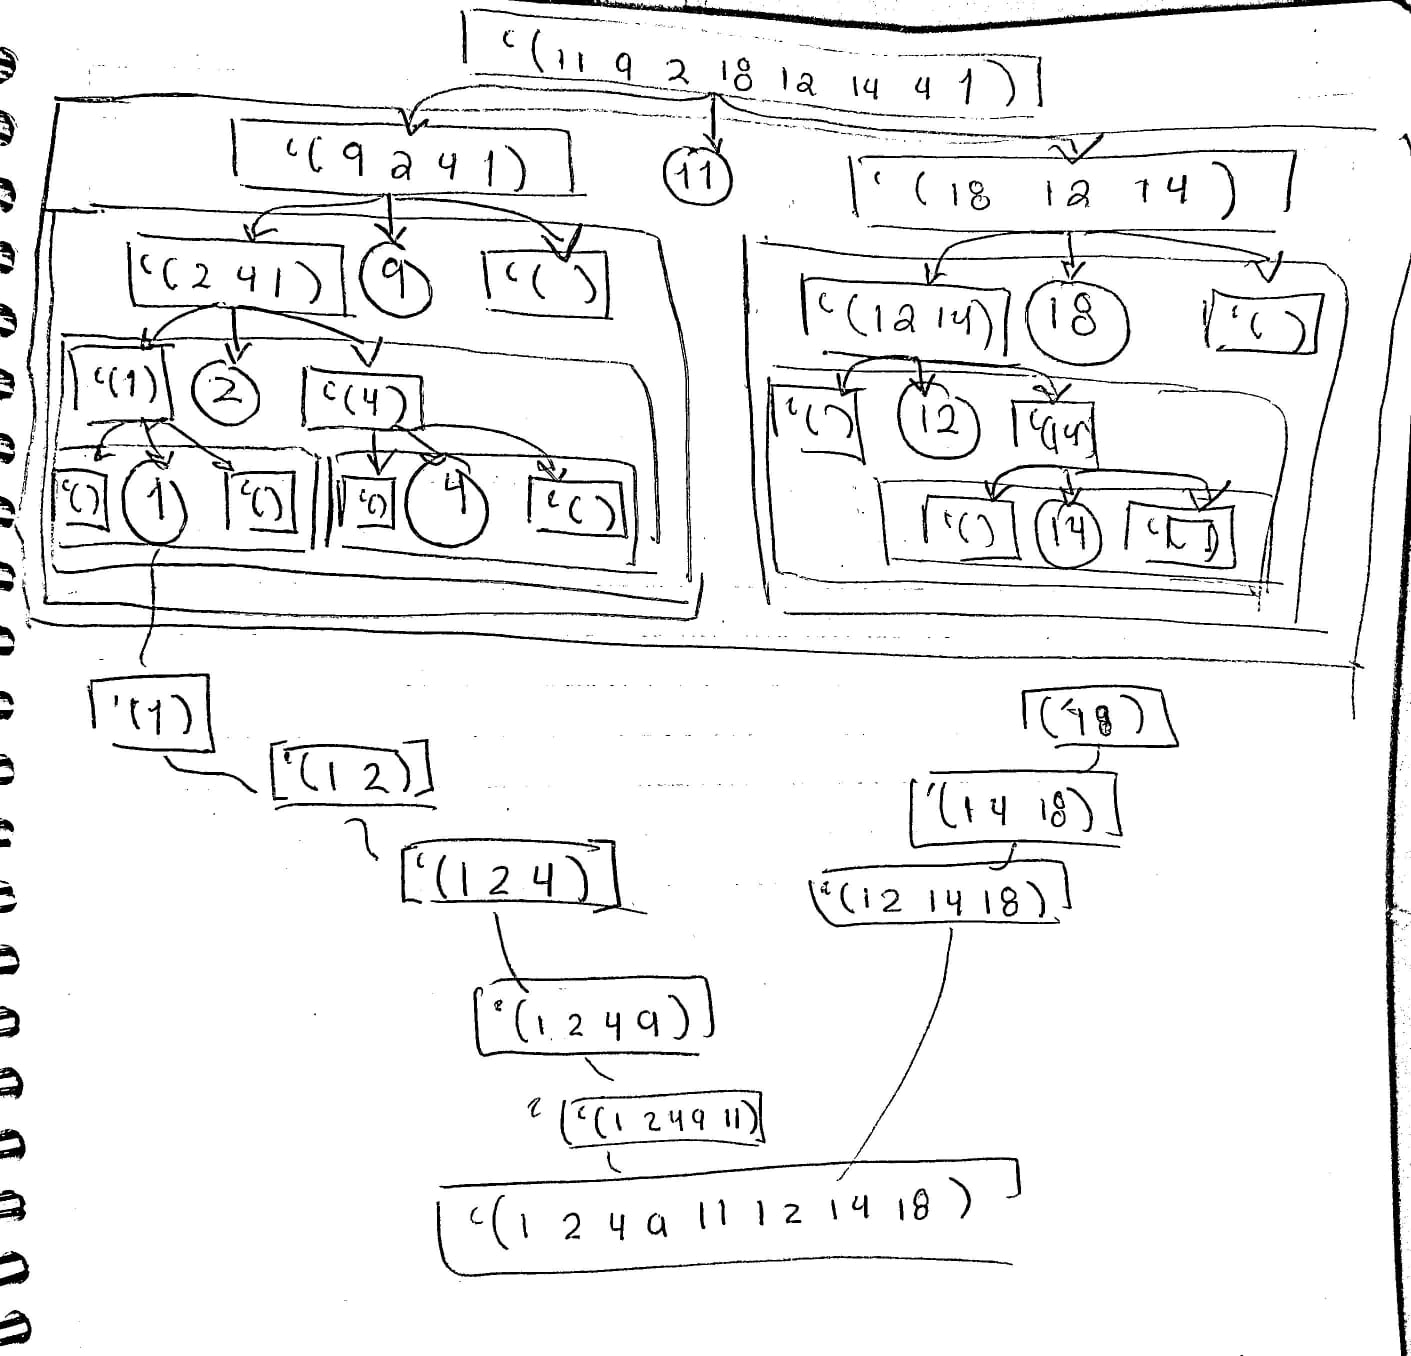
\includegraphics[width=15cm]{img}
\centering
\end{figure}

\newpage
\section*{Problema 11}
Si la entrada a quicksort contiene varias repeticiones de un número, va a regresar
una lista estrictamente más corta que la entrada. Responde el por qué y arregla el problema. \\ \\

La llamada recursiva de quicksort divide el problema (la lista) en 3 partes.
\begin{enumerate}
\item Los que son estrictamente menores al pivote.
\item El elemento
\item Los que son estrictamente mayores al pivote.
\end{enumerate}
\begin{lstlisting}[title=quicksort]
(define (quicksort ls)
  (cond
    [(empty? ls) null]
    [else
     (define pivot (first ls))
     (append (quicksort (smallers ls pivot))
             (list pivot)
             (quicksort (largers ls pivot)))]))
\end{lstlisting}

Una manera de solucionarlo puede ser que en la 2) parte en vez de solo seleccionar el pivote se construya una lista de todas las repeticiones del pivote.
\begin{lstlisting}[title=quicksort]
(define (quicksort ls)
  (cond
    [(empty? ls) null]
    [else
     (define pivot (first ls))
     (append (quicksort (smallers ls pivot))
             (filter (lambda (x) (equal? x pivot)) ls)
             (quicksort (largers ls pivot)))]))
\end{lstlisting}
\newpage
\section*{Problema 13}
Implementa una versión de quicksort que utilice isort si la longitud de la entrada está
por debajo de un umbral. Determina este umbral utilizando la función time , escribe el procedimiento
que seguiste para encontrar este umbral. \\

Para encontrar el umbral defino una lista de longitud n con elementos aleatorios, luego con $time$ comparo el tiempo de $isort$ y de $quicksort$.
\begin{lstlisting}[title= timing quicksort and isort]
(define (randlist n)
  (shuffle (range n)))
(define (greater x y) (> x y))

n=10,000
isort:     cpu time: 14729 real time: 14719 gc time: 2746
quicksort: cpu time:   136 real time:   136 gc time:   46

n=1000
isort:     cpu time: 154 real time: 155 gc time: 39
quicksort: cpu time:   8 real time:   8 gc time:  0

n=100
isort:     cpu time: 1 real time: 1 gc time: 0
quicksort: cpu time: 0 real time: 0 gc time: 0

\end{lstlisting}
Se toma que el Umbral = 100 ya que no hay diferencia entre un procedimiento con el otro.
\newpage
\section*{Problema 18}
Considera la siguiente definición de smallers , uno de los procedimientos utilizados
en quicksort , responde en qué puede fallar al utilizar esta versión modificada en el procedimiento
de ordenamiento.

\begin{lstlisting}[title = smallers]
(define (smallers l n)
  (cond
    [(empty? l) '()]
    [else (if (<= (first l) n)
              (cons (first l) (smallers (rest l) n))
              (smallers (rest l) n))]))
\end{lstlisting}

La llamada recursiva de quicksort divide el problema (la lista) en 3 partes.
\begin{enumerate}
\item Los que son estrictamente menores al pivote.
\item Los que son igual al elemento.
\item Los que son estrictamente mayores al pivote.
\end{enumerate}

Con esta modificación tenemos el problema de incluír al pivote dentro 1) y por tanto entrar en un bucle infinito.
\section*{Problema 19}
Describe con tus propias palabras cómo funciona find-largest-divisor de gcd-structural . Responde por qué comienza desde (min n m) .

\begin{lstlisting}[title = gcd-structural]
(define (gcd-structural n m)
  (define (find-largest-divisor k)
    (cond [(= i 1) 1]
          [(= (remainder n i) (remainder m i) 0) i]
          [else (find-largest-divisor (- k 1))]))
  (find-largest-divisor (min n m)))
\end{lstlisting}

Para encontrar el \textit{greatest common denominator} este algorítmo itera de uno en uno desde el mínimo de los 2 argumentos. Por ejemplo, para encontral el gdc de 100 y 40 checa si el min(100, 40) = 40 divide a ambos y no deja residuo (común denominador), si no es entonces prueba con el 39 y así sucesivamente.
\section*{Problema 20}
Describe con tus propias palabras cómo funciona find-largest-divisor de gcd-
generative .

\begin{lstlisting}[title = gcd-generative]
(define (gcd-generative n m)
  (define (find-largest-divisor max min)
    (if (= min 0)
        max
        (find-largest-divisor min (remainder max min))))
  (find-largest-divisor (max n m) (min n m)))
\end{lstlisting}

Es una implementación del algorítmo de Euclídes. Encontrar el $(gcd\,\, a, b)$ es encontrar el número más grande que divide $a$ y $b$, el caso trivial es cuando uno de los dos es 0. De otra forma se sabe, matemáticamente hablando, que al dividir por ejempo $ a$ con $b$ nos queda que $a = pb + r$, y  un número que divide a $b$ y $a$  debe dividir a $r$. Si $r=0$ (caso trivial) entonces el gdc es b. De otra forma encontrar el $(gcd\,\, b, r)$ nos dará el $(gcd\,\, a, b)$.

\section*{Problema 21}
Utiliza la función time para determinar cuál de las dos implementaciones es más
eficiente, escribiendo tu respuesta con los tiempos de ejecución obtenidos con ambos procedimientos
para valores “pequeños”, “medianos” y “grandes”. Justifica qué valores usaste en cada una de estas
mediciones y por qué los consideraste de ese “tamaño”. \\ \\

Dado que es structural es iterativo, un primo lo suficientemente grande va a ser que tenga un mal tiempo, ya que basicamente se va a reducir a que cuente hacia atras desde ese primo:
\begin{lstlisting}[title= gcd: structural vs generative]
PRIMES
n=1259, m=1889
structural: cpu time: 0 real time: 0 gc time: 0
generative: cpu time: 0 real time: 0 gc time: 0

n=241,271, m=31,397
structural: cpu time: 3 real time: 3 gc time: 0
generative: cpu time: 0 real time: 0 gc time: 0

n=13,466,917, m=6,972,593
structural: cpu time: 665 real time: 664 gc time: 0
generative: cpu time:   0 real time:   0 gc time: 0

n=43,112,609, m=37,156,667
structural: cpu time: 3598 real time: 3594 gc time: 0
generative: cpu time:    0 real time:    0 gc time: 0

n=243243243243232432432323432327 m=23)
structural: cpu time: 0 real time: 0 gc time: 0
generative: cpu time: 0 real time: 0 gc time: 0
\end{lstlisting}

Aquí se puede observar la eficiencia de generative aún para números grandes mientras que structural depende del mínimo y que sea primo obliga al algorítmo itere todo el número. \\ \\

Por otro lado, los números de Fibonacci deberían de ser la debilidad de generative:

\begin{lstlisting}[title= gcd: structural vs generative]
FIBONACCI
> (t 1259 1889)
cpu time: 0 real time: 0 gc time: 0
cpu time: 0 real time: 0 gc time: 0
1
> (t 241271 31397)
cpu time: 3 real time: 3 gc time: 0
cpu time: 0 real time: 0 gc time: 0
1
> (t 13466917 6972593)
cpu time: 665 real time: 664 gc time: 0
cpu time: 0 real time: 0 gc time: 0
1
> (t 43112609 37156667)
cpu time: 3598 real time: 3594 gc time: 0
cpu time: 0 real time: 0 gc time: 0
1
> (t 57885161 13)
cpu time: 0 real time: 0 gc time: 0
cpu time: 0 real time: 0 gc time: 0
1
> (t 82589933 19937)
cpu time: 2 real time: 2 gc time: 0
cpu time: 0 real time: 0 gc time: 0
1
> (t 8258993 19932)
cpu time: 2 real time: 2 gc time: 0
cpu time: 0 real time: 0 gc time: 0
1
> (t 8258992343243 4)
cpu time: 0 real time: 0 gc time: 0
cpu time: 0 real time: 0 gc time: 0
1
> (t 23432493242348324728374 3)
cpu time: 1 real time: 0 gc time: 0
cpu time: 0 real time: 0 gc time: 0
3
> (t 43274387468732465874326587432658327465873246587432 4)
cpu time: 0 real time: 0 gc time: 0
cpu time: 0 real time: 0 gc time: 0
4
> (t 32482349837458235732465943287598327598327532324759843275843275432 3)
cpu time: 0 real time: 0 gc time: 0
cpu time: 0 real time: 0 gc time: 0
3
> (t 4283498273498273498279874329847298474982749287449742874724728749239874298743298742398749872398743298742987343298742987498732987432 2)
cpu time: 0 real time: 0 gc time: 0
cpu time: 0 real time: 0 gc time: 0
2
> (t 4324343243243243 3232)
cpu time: 1 real time: 0 gc time: 0
cpu time: 0 real time: 0 gc time: 0
1
> (t 243243243243232432432323432327 23)
cpu time: 0 real time: 0 gc time: 0
cpu time: 0 real time: 0 gc time: 0
1
\end{lstlisting}
Pero observamos que el remainder le hace todo el trabajo a generative y sigue siendo más eficiente, aún cuando aumento o disminuyo la distancia entre los parametros, cuando son fibonacci, fibonacci primos, fibonacci consecutivos, y otras variaciones. Por que el algóritmo de Euclídes, junto con una buena implementación de remainder, es exagerademente eficiente.
\section*{Problema 22}
Piensa y describe por qué no siempre es la mejor opción elegir el procedimiento más
eficiente en tiempo de ejecución. Utiliza criterios que no sean el de “eficiencia”. \\

\noindent Siguiendo la linea de pensamiento del epigráma de Alan Perlis: \\
"Simplicity does not precede complexity, but follows it." \\

Los casos donde  una solución elegante y eficiente por lo general son resultados de un complejo análisis derivado de otras áreas (matemáticas) por lo que para nosotros programadores promedio, es dificil entender porque funciona, en que casos se comporta mejor, en cuales no, etc. Por tanto es preferible, si no es un sistema crítico, que la solución o algorítmo sea aquel que podamos entender y desmenuzar nosotros mismos. \\
Los casos donde NO es una solución elegante pero es eficiente o se vale de "trucos" son dificiles de entender para quienes no estuvieron realizando esos "ajuste" que mejoraron el procedimiento.

Para ambos casos es mejor un algorítmo que describa el problema y su solución de manera entendible para quienes la implementan.

\end{document}
